\documentclass{beamer}
\mode<presentation>
% \usecolortheme{albatross}
\usetheme{Malmoe}
\useinnertheme{rectangles}
\useoutertheme{infolines}

\usepackage{graphicx}
\title{Autoencoders}
\author[Annada]{Annada Behera}
\date{\today}

\begin{document}

\begin{frame}
	\titlepage
\end{frame}

\begin{frame}
	\frametitle{What is a autoencoder?}
	\begin{itemize}
	\item An autoencoder\footnote{\url{https://en.wikipedia.org/wiki/Autoencoder}} is a artificial neural network that learns the efficient codings
	of unlabeled data.
	\item It works both as a discriminator and a generator.
	\end{itemize}
\end{frame}

\begin{frame}
	\begin{definition}
	\begin{itemize}

	\item Discriminator $p(y|x)$ estimates the probability of a label $y$ given an
	observation $x$.
	\item Generator $p(x|y)$ is the probability of observing $x$ for a optional label $y$.
	\end{itemize}
	\end{definition}
\end{frame}

\begin{frame}
	\begin{block}{Generator Framework}
	\begin{itemize}
		\item We have a set of observation $X$.
		\item We assume that the observation was generated by some unknown
		distribution $P_d$.
		\item Our aim is to generate a model $P_m$ that is as close to $P_d$
		as possible.
		\item We are happy with $P_m$ if
		\begin{itemize}
			\item The observations sampled from $P_m$ appears to be
			drawn from $P_d$.
			\item The observations sampled from $P_m$ is considerably
			different from $X$.
		\end{itemize}
	\end{itemize}
	\end{block}
\end{frame}

\begin{frame}
\frametitle{An example}
\begin{columns}
	\begin{column}{.5\linewidth}
		\begin{itemize}
			\item Given a set of observations $X$ in a very high dimensional
			sample space, they can be instead represented in a compact
			low dimensional space.
			\item Learning the low dimensional representation is called
			\textbf{representation learning}.
			\item The low dimensional representation is called \textbf{latent space}.
		\end{itemize}
	\end{column}
	\begin{column}{.5\linewidth}
		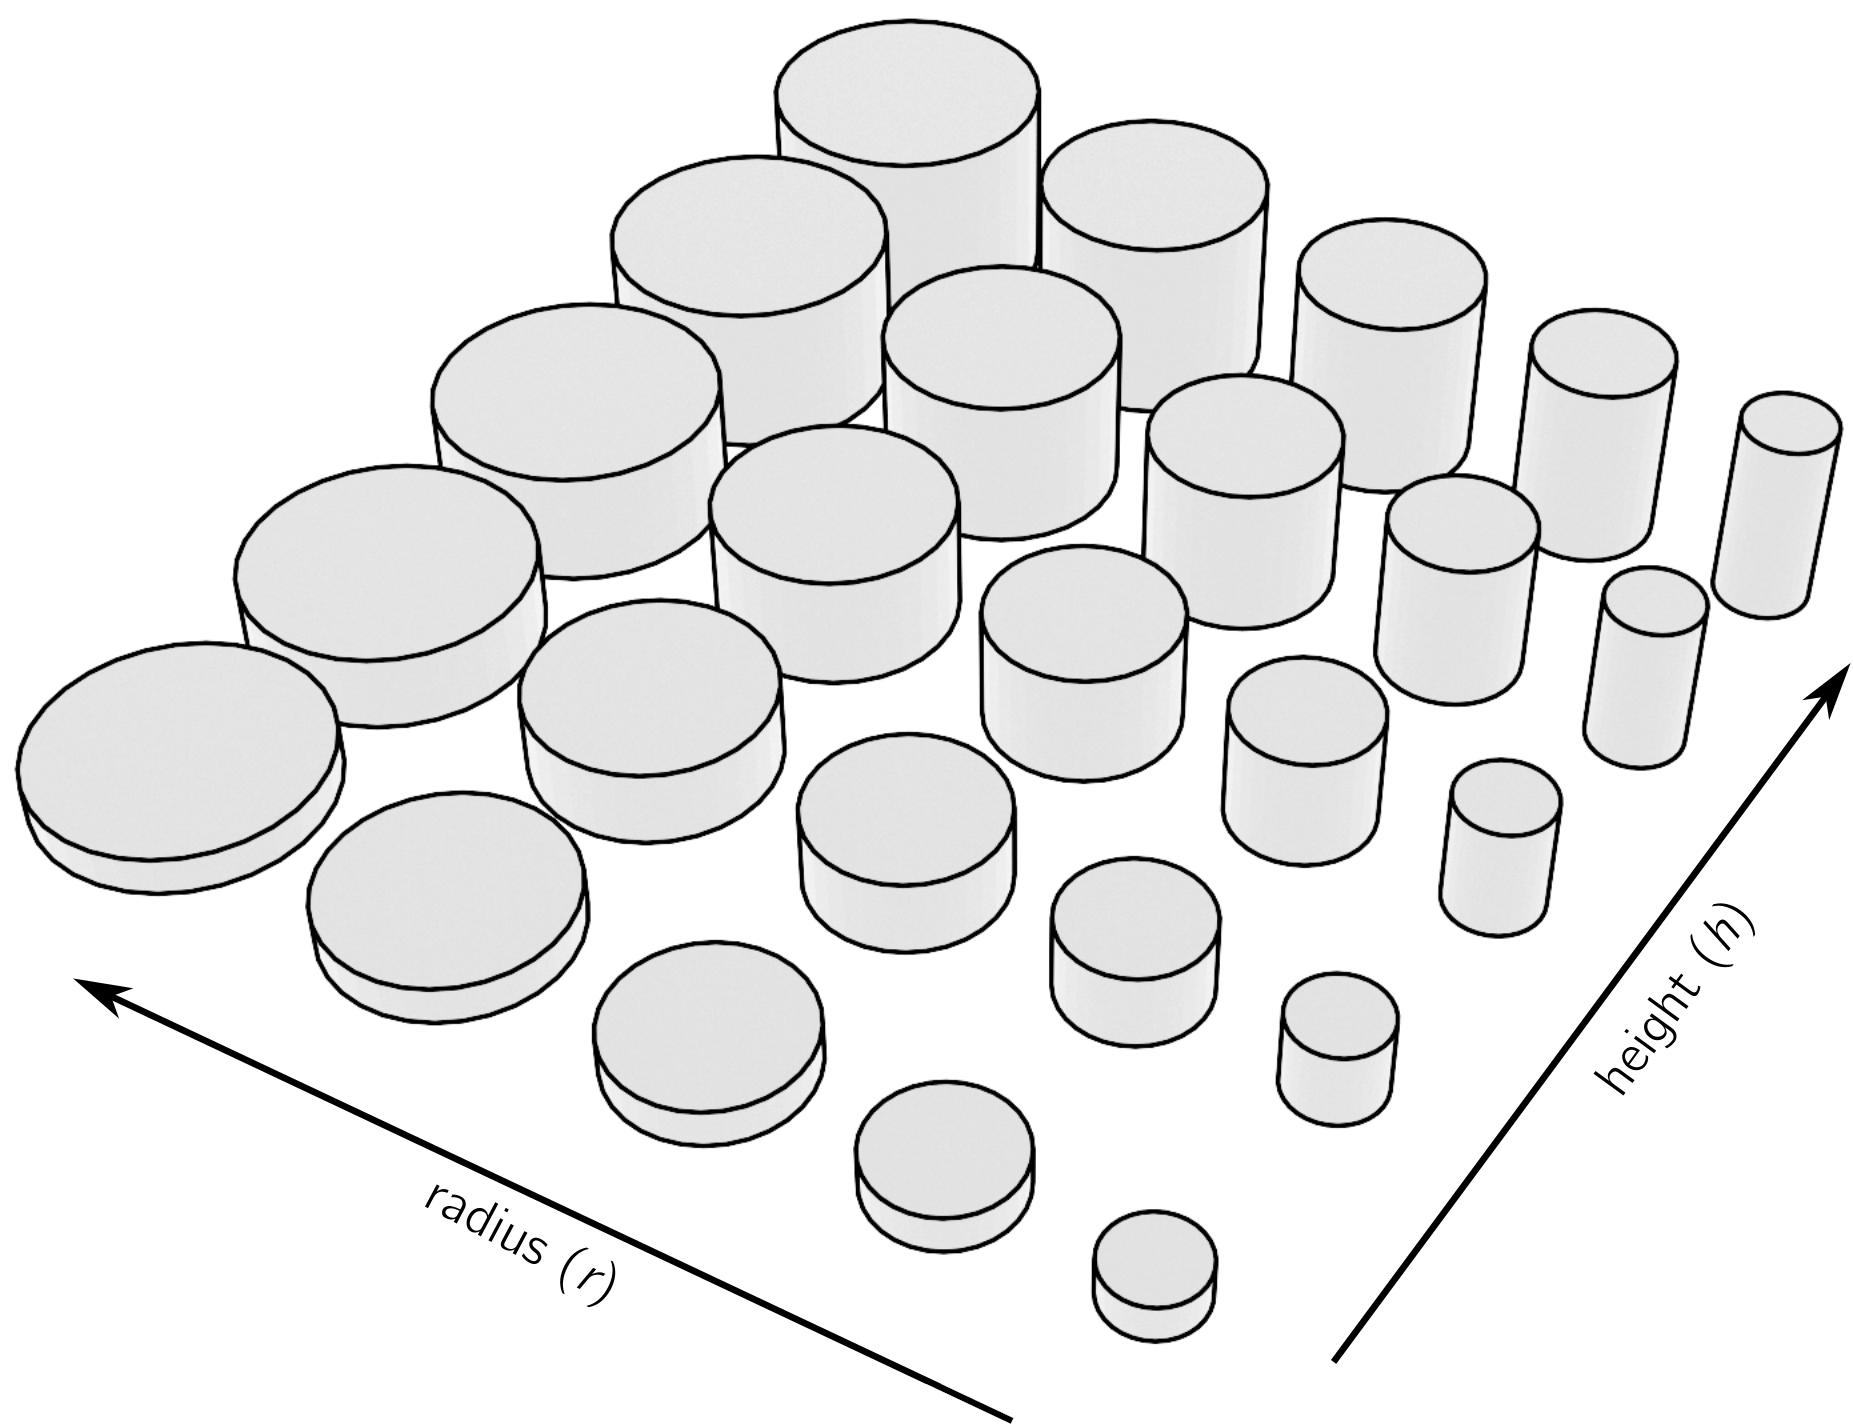
\includegraphics[width=\linewidth]{./example.png}
	\end{column}
\end{columns}
\end{frame}

\begin{frame}
\begin{definition}
	\begin{itemize}
		\item The sample space is the set of all observation $x$ can take,
		i.e, $X$.
		\item The probability density function, $p(x)$ is a function that
		maps a point in the sample space to a number between 0 and 1.
		\item An encoder $Enc(x)$ takes a high-dimensional input vector
		and ``compresses'' the data to a low dimensional output.
		\item A decoder, $Dec$ ``decompresses'' the data from low dimension to
		a high dimension.
	\end{itemize}
\end{definition}
\begin{equation}
	Enc:\mathbb{R}^m\to\mathbb{R}^n,\ Dec:\mathbb{R}^n\to\mathbb{R}^m\qquad m>>n
\end{equation}
\end{frame}

\begin{frame}
	\begin{definition}
		An autoencoder $AE:\mathbb{R}^n\to\mathbb{R}^n$ is defined as,
		\begin{equation}
			AE_\theta(x) = Dec_\theta(Enc_\theta(x))
		\end{equation}
		The $Enc$ and $Dec$ functions are both neural networks in our cases,
		but it is not necessary that they should be one.

		$\theta$ is the weights of the neural networks.
	\end{definition}
	\begin{center}
	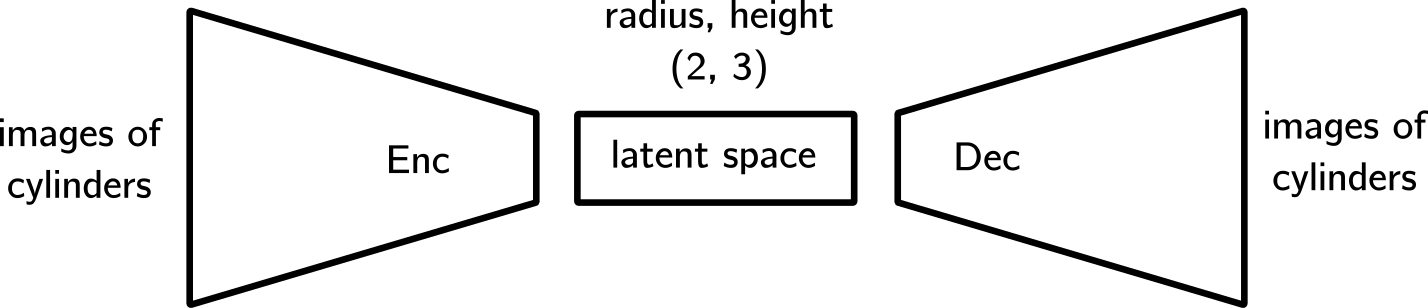
\includegraphics[width=.75\linewidth]{./encdec.png}
	\end{center}
\end{frame}

\begin{frame}
	\frametitle{The AE loss}
	The loss function is defined as, $\mathcal{L}(x,AE(x))$ is generally uses
	the RMSE loss, defined as,
	\begin{equation}
		RMSE(x,AE(x)) = \sqrt{\mathbb E[(x-AE(x))^2]}
	\end{equation}
	and the KL-divergence loss, 
	\begin{equation}
		D_{kl}(P_d,P_m) = \sum_{x\in X} P_d(x)\log\bigg(\frac{P_d(x)}{P_m(x)}\bigg)
	\end{equation}
\end{frame}

\end{document}
